% Options for packages loaded elsewhere
\PassOptionsToPackage{unicode}{hyperref}
\PassOptionsToPackage{hyphens}{url}
%
\documentclass[
  12 pt,
  a4paper,
]{article}
\usepackage{amsmath,amssymb}
\usepackage{setspace}
\usepackage{iftex}
\ifPDFTeX
  \usepackage[T1]{fontenc}
  \usepackage[utf8]{inputenc}
  \usepackage{textcomp} % provide euro and other symbols
\else % if luatex or xetex
  \usepackage{unicode-math} % this also loads fontspec
  \defaultfontfeatures{Scale=MatchLowercase}
  \defaultfontfeatures[\rmfamily]{Ligatures=TeX,Scale=1}
\fi
\usepackage{lmodern}
\ifPDFTeX\else
  % xetex/luatex font selection
  \setmainfont[]{Times New Roman}
\fi
% Use upquote if available, for straight quotes in verbatim environments
\IfFileExists{upquote.sty}{\usepackage{upquote}}{}
\IfFileExists{microtype.sty}{% use microtype if available
  \usepackage[]{microtype}
  \UseMicrotypeSet[protrusion]{basicmath} % disable protrusion for tt fonts
}{}
\makeatletter
\@ifundefined{KOMAClassName}{% if non-KOMA class
  \IfFileExists{parskip.sty}{%
    \usepackage{parskip}
  }{% else
    \setlength{\parindent}{0pt}
    \setlength{\parskip}{6pt plus 2pt minus 1pt}}
}{% if KOMA class
  \KOMAoptions{parskip=half}}
\makeatother
\usepackage{xcolor}
\usepackage[margin=1in]{geometry}
\usepackage{color}
\usepackage{fancyvrb}
\newcommand{\VerbBar}{|}
\newcommand{\VERB}{\Verb[commandchars=\\\{\}]}
\DefineVerbatimEnvironment{Highlighting}{Verbatim}{commandchars=\\\{\}}
% Add ',fontsize=\small' for more characters per line
\usepackage{framed}
\definecolor{shadecolor}{RGB}{248,248,248}
\newenvironment{Shaded}{\begin{snugshade}}{\end{snugshade}}
\newcommand{\AlertTok}[1]{\textcolor[rgb]{0.94,0.16,0.16}{#1}}
\newcommand{\AnnotationTok}[1]{\textcolor[rgb]{0.56,0.35,0.01}{\textbf{\textit{#1}}}}
\newcommand{\AttributeTok}[1]{\textcolor[rgb]{0.13,0.29,0.53}{#1}}
\newcommand{\BaseNTok}[1]{\textcolor[rgb]{0.00,0.00,0.81}{#1}}
\newcommand{\BuiltInTok}[1]{#1}
\newcommand{\CharTok}[1]{\textcolor[rgb]{0.31,0.60,0.02}{#1}}
\newcommand{\CommentTok}[1]{\textcolor[rgb]{0.56,0.35,0.01}{\textit{#1}}}
\newcommand{\CommentVarTok}[1]{\textcolor[rgb]{0.56,0.35,0.01}{\textbf{\textit{#1}}}}
\newcommand{\ConstantTok}[1]{\textcolor[rgb]{0.56,0.35,0.01}{#1}}
\newcommand{\ControlFlowTok}[1]{\textcolor[rgb]{0.13,0.29,0.53}{\textbf{#1}}}
\newcommand{\DataTypeTok}[1]{\textcolor[rgb]{0.13,0.29,0.53}{#1}}
\newcommand{\DecValTok}[1]{\textcolor[rgb]{0.00,0.00,0.81}{#1}}
\newcommand{\DocumentationTok}[1]{\textcolor[rgb]{0.56,0.35,0.01}{\textbf{\textit{#1}}}}
\newcommand{\ErrorTok}[1]{\textcolor[rgb]{0.64,0.00,0.00}{\textbf{#1}}}
\newcommand{\ExtensionTok}[1]{#1}
\newcommand{\FloatTok}[1]{\textcolor[rgb]{0.00,0.00,0.81}{#1}}
\newcommand{\FunctionTok}[1]{\textcolor[rgb]{0.13,0.29,0.53}{\textbf{#1}}}
\newcommand{\ImportTok}[1]{#1}
\newcommand{\InformationTok}[1]{\textcolor[rgb]{0.56,0.35,0.01}{\textbf{\textit{#1}}}}
\newcommand{\KeywordTok}[1]{\textcolor[rgb]{0.13,0.29,0.53}{\textbf{#1}}}
\newcommand{\NormalTok}[1]{#1}
\newcommand{\OperatorTok}[1]{\textcolor[rgb]{0.81,0.36,0.00}{\textbf{#1}}}
\newcommand{\OtherTok}[1]{\textcolor[rgb]{0.56,0.35,0.01}{#1}}
\newcommand{\PreprocessorTok}[1]{\textcolor[rgb]{0.56,0.35,0.01}{\textit{#1}}}
\newcommand{\RegionMarkerTok}[1]{#1}
\newcommand{\SpecialCharTok}[1]{\textcolor[rgb]{0.81,0.36,0.00}{\textbf{#1}}}
\newcommand{\SpecialStringTok}[1]{\textcolor[rgb]{0.31,0.60,0.02}{#1}}
\newcommand{\StringTok}[1]{\textcolor[rgb]{0.31,0.60,0.02}{#1}}
\newcommand{\VariableTok}[1]{\textcolor[rgb]{0.00,0.00,0.00}{#1}}
\newcommand{\VerbatimStringTok}[1]{\textcolor[rgb]{0.31,0.60,0.02}{#1}}
\newcommand{\WarningTok}[1]{\textcolor[rgb]{0.56,0.35,0.01}{\textbf{\textit{#1}}}}
\usepackage{graphicx}
\makeatletter
\def\maxwidth{\ifdim\Gin@nat@width>\linewidth\linewidth\else\Gin@nat@width\fi}
\def\maxheight{\ifdim\Gin@nat@height>\textheight\textheight\else\Gin@nat@height\fi}
\makeatother
% Scale images if necessary, so that they will not overflow the page
% margins by default, and it is still possible to overwrite the defaults
% using explicit options in \includegraphics[width, height, ...]{}
\setkeys{Gin}{width=\maxwidth,height=\maxheight,keepaspectratio}
% Set default figure placement to htbp
\makeatletter
\def\fps@figure{htbp}
\makeatother
\setlength{\emergencystretch}{3em} % prevent overfull lines
\providecommand{\tightlist}{%
  \setlength{\itemsep}{0pt}\setlength{\parskip}{0pt}}
\setcounter{secnumdepth}{-\maxdimen} % remove section numbering
\ifLuaTeX
\usepackage[bidi=basic]{babel}
\else
\usepackage[bidi=default]{babel}
\fi
\babelprovide[main,import]{spanish}
\ifPDFTeX
\else
\babelfont{rm}[]{Times New Roman}
\fi
% get rid of language-specific shorthands (see #6817):
\let\LanguageShortHands\languageshorthands
\def\languageshorthands#1{}
\ifLuaTeX
  \usepackage{selnolig}  % disable illegal ligatures
\fi
\usepackage{bookmark}
\IfFileExists{xurl.sty}{\usepackage{xurl}}{} % add URL line breaks if available
\urlstyle{same}
\hypersetup{
  pdfauthor={Tomàs Ferrandis Moscardó},
  pdflang={es-ES},
  hidelinks,
  pdfcreator={LaTeX via pandoc}}

\title{U7-OpenLDAP-2}
\usepackage{etoolbox}
\makeatletter
\providecommand{\subtitle}[1]{% add subtitle to \maketitle
  \apptocmd{\@title}{\par {\large #1 \par}}{}{}
}
\makeatother
\subtitle{Autenticar i perfils}
\author{Tomàs Ferrandis Moscardó}
\date{}

\begin{document}
\maketitle

{
\setcounter{tocdepth}{2}
\tableofcontents
}
\setstretch{1.5}
\section{1 Autenticació basada en
LDAP}\label{autenticaciuxf3-basada-en-ldap}

\subsection{1.1 Introducció}\label{introducciuxf3}

Ara estudiarem autenticar en Linux els usuaris en en servidor LDAP
enlloc utilitzar els clàssics fitxers /etc/passwd, /etc/group i
/etc/shadow. Per fer-ho hem d'instal·lar i configurar els paquets
\textbf{libpam-ldap} i \textbf{libnss-ldap}.

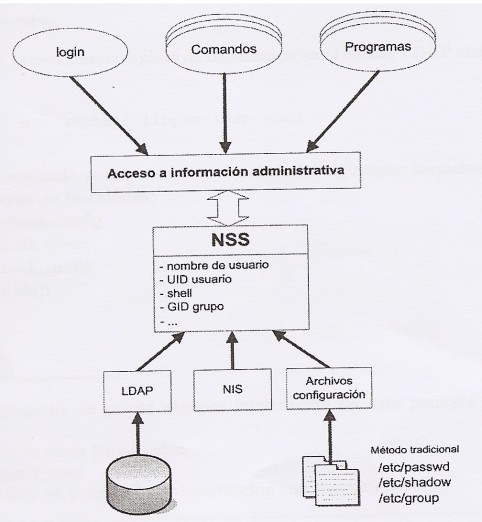
\includegraphics{png/nss.png}

\subsection{1.2 Llibreries d'autenticació pam-ldap i
nss-ldap}\label{llibreries-dautenticaciuxf3-pam-ldap-i-nss-ldap}

La llibreria \textbf{pam-ldap} permet que les aplicacions que utilitzen
PAM (Pluggable Authentication Modules) per autenticar, puguen fer-ho
mitjançant un servidor LDAP. Linux empra aquest mecanisme per a la
validació local, per tant ens cal instal·lar aquesta llibreria.

L'arxiu de configuració d'aquesta llibreria és \textbf{/etc/ldap.conf}.
Hi ha altres aplicacions o serveis que utilitzen PAM per l'autenticació
i per tant podrien, gràcies a la llibreria pam-ldap, autenticar-se
davant un servidor LDAP. Per especificar el mode d'autenticació de cada
servei és necessari configurar els arxius que es troben a la carpeta
\textbf{/etc/pam.d/}. Al final d'aquest apartat s'indiquen els canvis
necessaris en aquests arxius. La llibreria \textbf{nss-ldap} permet que
un servidor LDAP \textbf{suplanti als arxius /etc/passwd, /etc/group i
/etc/shadow} com a bases de dades del nostre sistema client. El seu
arxiu de configuració es troba a \textbf{/etc/ldap.conf} (comparteix
arxiu de configuració amb la llibreria pam-ldap).

Posteriorment haurem de configurar el arxius que són
\textbf{/etc/nsswitch.conf} per a que s'utilitze LDAP com a base de
dades del sistema en lloc dels arxius passwd, group i shadow.

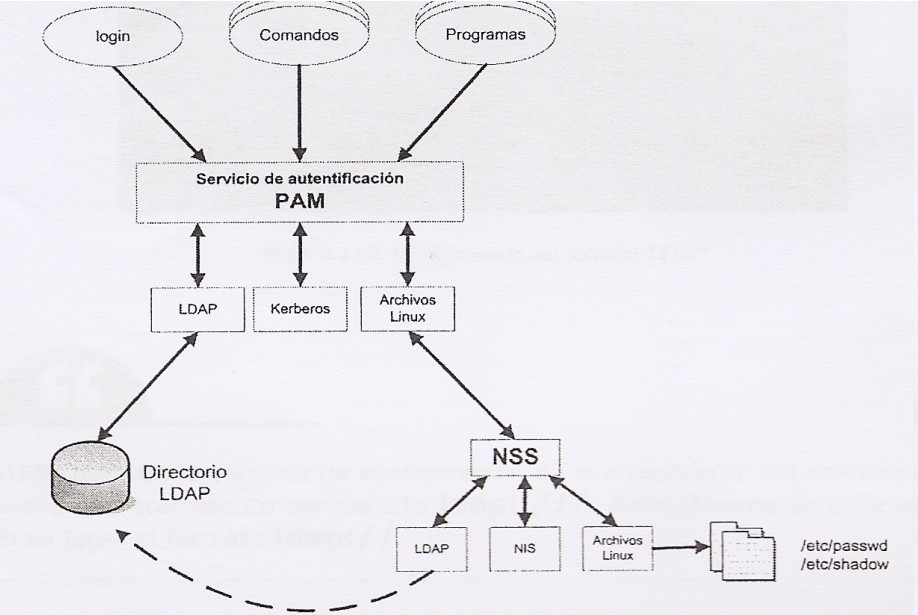
\includegraphics{png/pam.png}

\subsection{1.3 Instal·lació i configuració de libpam-ldap i
libnss-ldap}\label{installaciuxf3-i-configuraciuxf3-de-libpam-ldap-i-libnss-ldap}

\textbf{Client}

\begin{Shaded}
\begin{Highlighting}[]
\FunctionTok{sudo}\NormalTok{ apt update}
\FunctionTok{sudo}\NormalTok{ apt upgrade}
\end{Highlighting}
\end{Shaded}

Instal·lem els paquets del client LDAP

\begin{Shaded}
\begin{Highlighting}[]
\FunctionTok{sudo}\NormalTok{ apt install libnss{-}ldap libpam{-}ldap ldap{-}utils }\AttributeTok{{-}y}
\end{Highlighting}
\end{Shaded}

Fixeu-vos que NO és ldapi:///, heu de llevar la ``i'' i la tercera
``/'', \url{ldap://192.168.10.1}

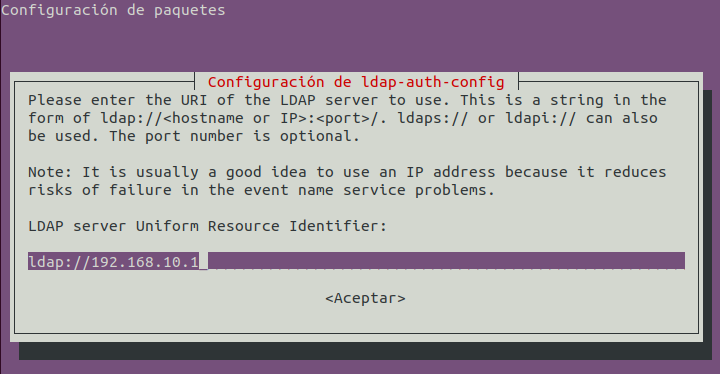
\includegraphics{png/libpam1.png}

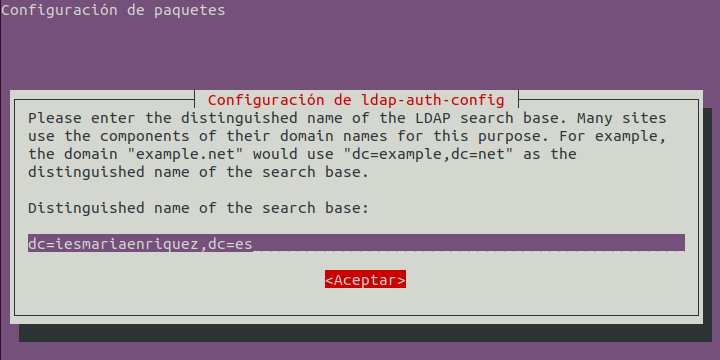
\includegraphics{png/libpam2.png}

A les següent 3 pantalles deixarem les opcions per defecte:

\begin{itemize}
\item
  LDAP version: 3
\item
  Make local root Database admin: Si
\item
  Does the LDAP database require login? No
\end{itemize}

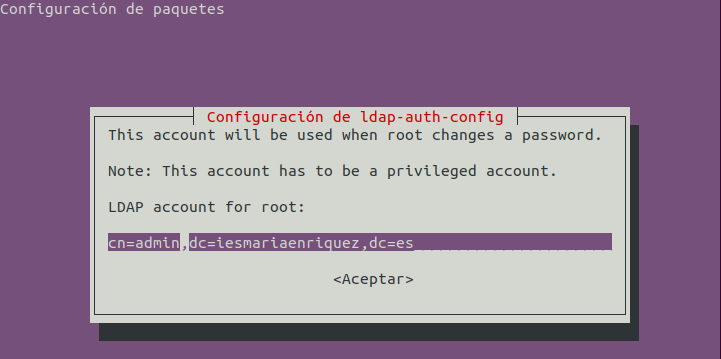
\includegraphics{png/libpam3.png}

La configuració que acabem de fer s'emmagatzema en el fitxer
\textbf{/etc/ldap.conf} el qual podem modificar manualment. Aquest
s'utilitza tant pel servei d'autenticació PAM com pel servei de noms NSS
(Name Service Switch). Si posteriorment tinguem que canviar aquesta
configuració podem editar el fitxer o, més fàcilment, el reconfigurarem
amb l'ordre \textbf{dpkg-reconfigure ldap-auth-config}.

\subsubsection{1.3.1 Configuració de NSS}\label{configuraciuxf3-de-nss}

\textbf{Client}

Per a que el servidor LDAP actue com si es tractara dels arxius passwd,
group i shadow, a més d'instal·lar les dos llibreries anteriors, hem
d'indicar que s'utilitze LDAP com alternativa per a autenticar usuaris.
Per a això modifiquem l'arxiu /etc/nsswitch.conf:

\begin{Shaded}
\begin{Highlighting}[]
\FunctionTok{sudo}\NormalTok{ nano /etc/nsswitch.conf}
\end{Highlighting}
\end{Shaded}

Únicament cal afegir ldap (no cal canviar compat per file systemd).
Segons la versió del client en les línies de passwd, group i shadow
posarà files, compat o files systemd. Els dos paràmetres signifiquen
pràcticament el mateix.

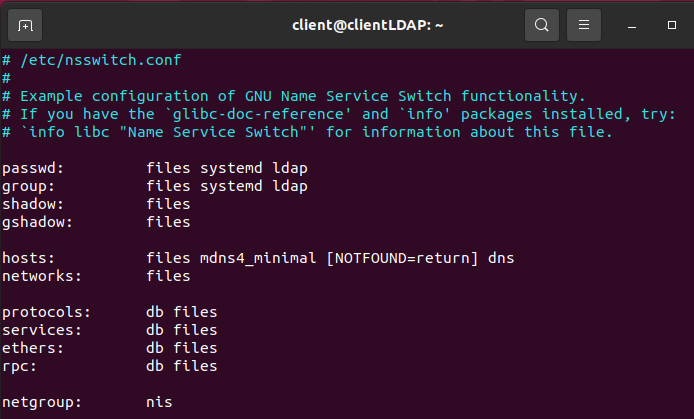
\includegraphics{png/libpam4.png}

Ací estem configurant que en primer lloc busque usuaris, grups i
contrasenyes en els fitxers locals i si no els troba busque en LDAP.

Respecte a les màquines (hosts) primer les busca en el fitxer local
(/etc/hosts) i si no les troba pregunta al DNS.

\begin{quote}
Si afegim ``ldap'' com últim element tant de passwd i group, a l'hora de
montar les carpetes, tindrà prioritat els directoris locals dels usuari
que les de LDAP.

Això ens pot portar problemes en la posterior configuració dels perfils
mòbils. Quan canviem la ruta del directori de cada usuari per a que el
perfil es dese al servidor.
\end{quote}

Actualitzem els canvis reiniciant la màquina o amb la següent ordre que
caldria instal·lar prèviament:

\begin{Shaded}
\begin{Highlighting}[]
\FunctionTok{sudo}\NormalTok{ nss\_updatedb ldap}
\end{Highlighting}
\end{Shaded}

\textbf{getent}

Amb ens mostra tant els usuaris locals com els creat en LDAP si NSS està
funcionant. És la foram de comprovar-ho.

\begin{Shaded}
\begin{Highlighting}[]
\FunctionTok{getent}\NormalTok{ passwd}
\end{Highlighting}
\end{Shaded}

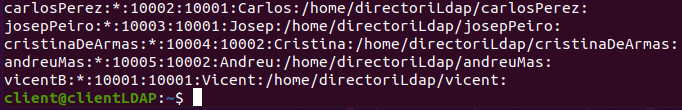
\includegraphics{png/libpam5.png}

Podeu consultar /var/log/auth.log

\subsubsection{1.3.2 Configuració de serveis
PAM}\label{configuraciuxf3-de-serveis-pam}

\textbf{Client}

Ara el nostre Linux ja estaria preparat per a autenticar-se com a LDAP.
Editant els fitxers que hi ha a la carpeta \textbf{/etc/pam.d} podem
configurar la forma en que s'autentica cadascun dels serveis que
requereixen autenticació. Per a no haver de fer-ho individualment,
existeixen uns arxius el nom dels quals comença per ``common'' i que en
molts d'aquests arxius hi fan referència mitjançant una línia
\texttt{@include}

\begin{itemize}
\item
  /etc/pam.d/common-auth (per a autenticar-se)
\item
  /etc/pam.d/common-account (per a disposar d'un compte)
\item
  /etc/pam.d/common-session (per a poder iniciar sessió)
\item
  /etc/pam.d/common-password (per a poder canviar la paraula de pas)
\end{itemize}

Aquest arxius contenen una línia que fa referència a la llibreria
\textbf{pam\_unix.so}, que correspon a l'autenticació contra els arxius
Linux (/etc/passwd, /etc/shadow,etc).

Observeu que el nostre sistema empra primer les llibreries
\textbf{pam\_ldap.so} per a autenticar els usuaris, i desprès les de
Linux.

Així, si la autenticació falla provarà amb els usuaris locals de Linux.

\begin{Shaded}
\begin{Highlighting}[]
\FunctionTok{sudo}\NormalTok{ nano /etc/pam.d/common{-}password}
\end{Highlighting}
\end{Shaded}

Aneu a la línia 26 i esborreu use\_authtok:

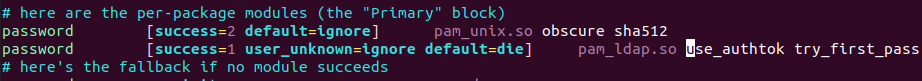
\includegraphics{png/libpam6.png}

Quedará així:

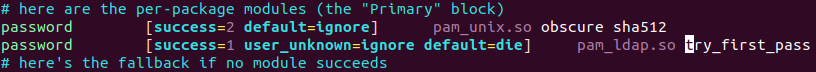
\includegraphics{png/libpam7.png}

\subsubsection{4.3.3 Creació automàtica directoris d'usuari
(home)}\label{creaciuxf3-automuxe0tica-directoris-dusuari-home}

\textbf{Client}

El mòdul \textbf{pam\_mkhomedir.so} és el que permet crear el directori
d'usuari.

\begin{itemize}
\tightlist
\item
  \emph{umask} indica els permisos aplicats.
\end{itemize}

Si umask=022, els permisos seran: 777 - 022 = 755 = rwx r-x r-x

\begin{itemize}
\tightlist
\item
  \emph{skel} ens indica un directori, el contingut del qual, es copiarà
  al nou directori d'usuari; pots posar-hi el que vullgues, tot es
  copiarà al nou directori HOME creat.
\end{itemize}

\begin{Shaded}
\begin{Highlighting}[]
\FunctionTok{sudo}\NormalTok{ nano /etc/pam.d/common{-}session}
\end{Highlighting}
\end{Shaded}

Baix de session optional pam\_system.so posem:

\begin{verbatim}
session optional pam_mkhomedir.so skel=/etc/skel umask=077
\end{verbatim}

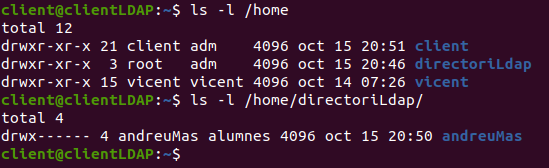
\includegraphics{png/libpam9.png}

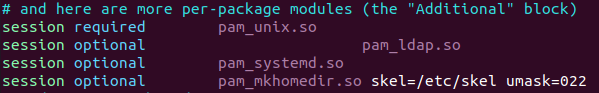
\includegraphics{png/libpam10.png}

És una bona pràctica per introduir un fitxer de informació sobre els
permisos, o que avise que estan utilitzant el servei LDAP, o el que
necessitem. Com hem ficat umask=077 els permisos que tindran per defecte
els directoris /home/usuari seran rwx --- ---

\begin{itemize}
\item
  client i vicent, son usuaris locals, la màscara per defecte és 022
  (0022)
\item
  andreuMas és un usuari LDAP, quan vam iniciar sessió per primera volta
  la màscara era 077
\end{itemize}

Si volem que els permisos per defecte dels nous directoris /home/usuari
siga rwx r-x r-x (els permisos habituals per als nous usuaris a Linux),
al fitxer hauríem de ficar umask=022. Per tant, ho deixarem així:

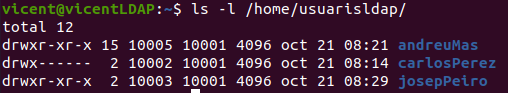
\includegraphics{png/libpam11.png}

Perquè els permisos queden com cal, podem canviar-los manualment amb
``chmod'' o bé eliminar la carpeta de l'usuari (cosa que causarà que
s'esborren totes les seues dades). Com podeu vore, els usuaris andreuMas
i josepPeiro s'han creat després d'haver fet el canvi del umask, en
canvi, carlosPerez manté els permisos del umask antic, cal canviar-los
per deixar-los com els d'un usuari

Per finalitzar la configuració i que s'apliquen els canvis del client,
reiniciem la màquina:

\begin{Shaded}
\begin{Highlighting}[]
\ExtensionTok{reboot}
\end{Highlighting}
\end{Shaded}

Si volem mostrar tots els usuaris dels llocs indicats a nsswitch.conf:
``compat/files'' i ``ldap'' farem:

\begin{Shaded}
\begin{Highlighting}[]
\FunctionTok{getent}\NormalTok{ passwd}
\end{Highlighting}
\end{Shaded}

\section{2 Perfils mòbils}\label{perfils-muxf2bils}

Ja coneixeu de Windows Server el concepte de Perfil Mòbil, no cal
repetir-lo. Ara que tenim configurat el directori LDAP podem
implementar-lo en el Ubuntu Server.

\subsection{2.1 Servidor}\label{servidor}

Cal fer que: * les carpetes personals dels usuaris s'allotgen al
servidor i * es munten automàticament en els clients en iniciar sessió.

Els passos a fer són:

\begin{enumerate}
\def\labelenumi{\arabic{enumi}.}
\item
  Creeu una subcarpeta en el servidor on emmagatzemar els homes.
  Exemple: /home/usuarisldap (si useu directament /home les exportacions
  i canvis que feu afectaran també als usuaris locals del servidor)
\item
  Compartiu-la en xarxa amb \textbf{NFS (Network File System)} amb
  permisos de lectura i escriptura per a tots els clients.
\end{enumerate}

Si no tenim instal·lat NFS:

\begin{Shaded}
\begin{Highlighting}[]
\FunctionTok{sudo}\NormalTok{ apt install nfs{-}kernel{-}server}
\end{Highlighting}
\end{Shaded}

El punt 2 consisteix en modificar el fitxer /etc/exports i afegir la
següent línia:

\begin{verbatim}
/home/usuarisldap *(rw,sync,no_root_squash,no_subtree_check) 
\end{verbatim}

Explicarem més avant el NFS.

Ara cal reiniciar el servidor.

\subsection{2.2 Client}\label{client}

Cal crear una carpeta que contindrà els continguts que es guarden de
cada usuari al serverLDAP.

Per fer-ho fàcil, anem a crearla a la mateixa ubicació
``/home/usuarisldap'' i li donem permisos complets al directori ``chmod
777'' el que ve a ser ``drwxrwxrwx''.

Fet això, anem a montar mitjançant el fitxer ``/etc/fstab'', que la
carpeta ubicada al servidor es muntarà de forma automàtica en el arranc
del sistema al nostre directori local.

Cal \textbf{instal·lar el paquet ``nfs-common''} perquè el fstab monte
correctament el directori allotjat al servidor, si no, voreu com no
funciona, accedireu a /home/usuarisldap i dins sols tindreu els
documents locals (no cap).

Per tant, com que tenim el servidor amb la IP: 192.168.10.1 i la carpeta
està ubicada a /home/usuarisldap, anem a afegir la següent línia al
fitxer /etc/fstab on bàsicament indiquem que la carpeta
``/home/usuarisldap'' de l'equip remot amb IP 192.168.10.1, es muntarà a
la carpeta local ``/home/usuarisldap'':

\begin{verbatim}
192.168.10.1:/home/usuarisldap /home/usuarisldap nfs auto,noatime,nolock,bg,nfsvers=3, intr,tcp,actimeo=1800 0 0
\end{verbatim}

Quedaria així:

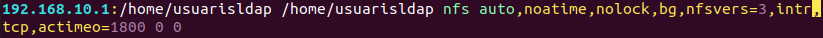
\includegraphics{png/perfilmobil1.png}

I per últim, cal que actualitzem a cadascun dels usuaris, la ruta del
seu directori per a què coincidisca amb la carpeta mòbil.

Des del jXplorer per exemple:

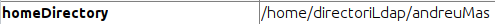
\includegraphics{png/perfilmobil2.png}

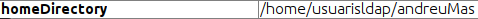
\includegraphics{png/perfilmobil3.png}

\begin{quote}
Quan el sistema detecta 2 ``homeDirectory'' per a un mateix usuari,
agafarà el directori més antic ( que és el local )
\end{quote}

\begin{quote}
Dos solucions:
\end{quote}

\begin{quote}
\begin{enumerate}
\def\labelenumi{\arabic{enumi}.}
\item
  Modificar en el fitxer ``nsswitch.conf'' l'ordre en que ``passwd'' i
  ``group'' revisarà els comptes d'usuari. Actualment l'ordre és
  ``files'' -\textgreater{} ``systemd'' -\textgreater{} ``ldap''.
  Canviar per: ``ldap'' -\textgreater{} ``files'' -\textgreater{}
  ``systemd'' Reiniciar la màquina perquè agafe les últimes dades
  actualitzades del servidor LDAP.
\item
  Eliminar el directori local (/home/directoriLdap) perquè LDAP funcione
  correctament.
\end{enumerate}
\end{quote}

Finalment, per verificar que tot està funcionant correctament, deuríem
de revisar fent ``login'' mitjançant un escriptori secundari de ubuntu
(``tty3'' per exemple) i revisant que quan iniciem sessió, crea
automàticament la carpeta que està al servidor. Exemple de andreuMas que
no tenia cap directori antic:

Des d'este moment tot el que creem amb eixe usuari, realment està
guardant-se al servidor, i es connecte des del client que es connecte
tindrà exactament el mateix.

\begin{quote}
El servidor deu estar operatiu quan el client arranque el servidor, si
no, fallarà el muntatge del directori NFS.
\end{quote}

\end{document}
